\documentclass[10pt]{beamer}
\usetheme{metropolis}

\usepackage{amsmath, booktabs, fontawesome5, natbib, subfigure, xcolor}

\usepackage[font=small,skip=0pt]{caption}

\usepackage{pgfplots}
\usepgfplotslibrary{dateplot}

\usepackage{xspace}
\newcommand{\themename}{\textbf{\textsc{metropolis}}\xspace}

\usepackage{graphicx}
\graphicspath{{../imgs/}}

\usepackage[T1]{fontenc}
\usepackage[french]{babel}

\usepackage{appendixnumberbeamer}

\usepackage{tikz}
\usetikzlibrary{shapes.geometric, arrows}
\tikzstyle{rect} = [rectangle, rounded corners, minimum width=2cm, minimum height=1.5cm, text centered, draw=black, fill=black!30]
\tikzstyle{squa} = [square, rounded corners, minimum width=1.25cm, minimum height=1.25cm, text centered, draw=black, fill=black!30]
\tikzstyle{elli} = [ellipse, minimum width=1.25cm, minimum height=1cm, text centered, draw=black, fill=black!30]
\tikzstyle{circ} = [circle, minimum width=1cm, minimum height=1cm, text centered, draw=black, fill=black!30]
\tikzstyle{arrow} = [thick,->,>=stealth]
\tikzstyle{drrow} = [thick,<->,>=stealth]
\tikzstyle{dline} = [dashed, ->, >=stealth]
\tikzstyle{dotted} = [densely dotted, ->, >=stealth]

\def\firstcircle{(90:1.75cm) circle (2.5cm)}
\def\secondcircle{(210:1.75cm) circle (2.5cm)}
\def\thirdcircle{(330:1.75cm) circle (2.5cm)}
\tikzset{fontscale/.style = {font=\relsize{#1}}}

\titlegraphic{\hfill\includegraphics[height=1.25cm]{~/Documents/scpobx/logo.pdf}}
\title{Méthodes des sciences sociales}
\subtitle{Séance 3 : Les types de données}
\author{Mickael Temporão}
\institute{\faEnvelope~$m.temporao@sciencespobordeaux.fr$\\\faTwitter~$@mickaeltemporao$}
\date{}

\begin{document}

\maketitle

\begin{frame}{Méthodes des sciences sociales}
    \begin{block}{Ordre du jour}
        \begin{itemize}
            \item[\faBook] Les types de données
            \item[\faFlask] Questions, méthode et données
            \item[\faLaptopCode] RStudio, \faRProject, \LaTeX
        \end{itemize}
    \end{block}
\end{frame}

\begin{frame}{\faExclamationTriangle~RAPPEL}
        \begin{block}{\faSlack~Slack}
            \begin{itemize}
                \item<2-> Installez l'application sur \faLaptop~et/ou \faMobile
                \item<3-> Si \faAt, alors \faReply
                \item<4-> Soyez actifs sur les \faHashtag channels
            \end{itemize}
        \end{block}
    \onslide<5->{
        \begin{block}{\faTools~Cours \& Outils}
            \begin{itemize}[<+->]
                \item Utilisez ces outils dans d'autres contextes
                \item Posez des questions sur les possibilités
                \item Demandez de l'aide si vous êtes bloqués
            \end{itemize}
        \end{block}
    }
\end{frame}

\section{\faBook~Théorie}

\begin{frame}{La sociologie positiviste (rappel)}
    \begin{block}{L'étude de la société basé sur l'observation systématique de comportements sociaux}
    \end{block}
    \begin{itemize}
        \item Importance de l'objectivité!
        \item Mettre de côté ses valeurs et croyances
        \item Approcher son objet d'étude comme un observateur neutre
        \item Se baser sur des preuves empiriques pour répondre à des questions sur le fonctionnement du monde social.
    \end{itemize}

    \begin{block}{Quel types de preuves empiriques?}
    \begin{itemize}
        \item Données quantitatives
        \item Données qualitatives
    \end{itemize}
    \end{block}
\end{frame}

\begin{frame}{La sociologie positiviste}
    \begin{block}{La recherche quantitative}
        La recherche quantitative se concentre sur l'étude de phénomènes sociaux observables dans le monde en utilisant généralement des données quantifiables et des modèles statistiques.
    \begin{itemize}
        \item L'objectif est de mesurer
        \item Données sous forme numérique
        \item Les informations peuvent être comptées \\(âge, revenu, ... mais aussi sexe, département...)
    \end{itemize}
    \end{block}

    \onslide<2>{
    On s'intéresse à mesurer l'effet d'une variable sur une autre:
    \begin{itemize}
        \item $Y = \alpha + \beta*x_i + \epsilon$
    \end{itemize}
}
\end{frame}

\begin{frame}{La sociologie positiviste}
    \begin{block}{La recherche qualitative}
        La recherche qualitative est l'étude de phénomènes sociaux observables plus difficilement quantifiables en se basant généralement sur des entretiens, questionnaires ou de l'observation participante ou non.
    \begin{itemize}
        \item L'objectif est d'illustrer ou de caractériser
        \item Données ne sont pas sous forme numérique
        \item L'information dont on a besoin ne peut être ou ne devrait pas être simplifié a un nombre dans un tableau
    \end{itemize}
    \end{block}

    \onslide<2>{
    On s'intéresse aux opinions et au valeurs latentes:
    \begin{itemize}
        \item Pourquoi certains citoyens refusent d'aller voter?
    \end{itemize}
}
\end{frame}

\begin{frame}{La sociologie positiviste}
    \begin{block}{Limites}
    Les études scientifiques impliquant des sujets humains et leur comportements viennent avec de nombreux défis.
    \begin{itemize}
        \item Ce qui nous intéresse n'est pas toujours observable
        \item Les humains ne sont pas toujours prévisibles
        \item Expériences difficilement contrôlables
        \item Implications éthiques
        \item On ne veut pas forcément modifier les conditions réelles
    \end{itemize}
    \end{block}
\end{frame}

\begin{frame}{La sociologie positiviste}
    \begin{columns}
        \begin{column}{0.5\textwidth}
            \begin{block}{Hawthorne Effect}
                \begin{itemize}
                    \item[\faBullseye] Améliorer la productivité des travailleurs
                    \item[\faVials] Expérience (Groupe contrôle/test)
                            \begin{itemize}
                                \item ajustement de l'éclairage
                                \item heures de travail
                                \item pauses
                            \end{itemize}
                \end{itemize}
            \end{block}
        \end{column}
    \begin{column}{0.5\textwidth}
        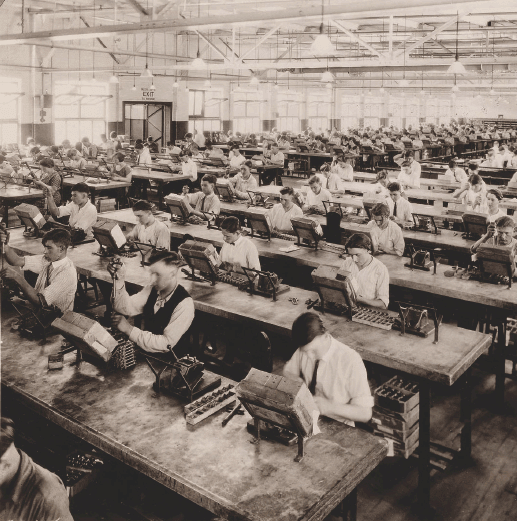
\includegraphics[width=\textwidth]{hawthorne}
        \begin{flushright}
            \small~Elton Mayo, 1920s
        \end{flushright}
    \end{column}
    \end{columns}
\end{frame}

\begin{frame}{Hawthorne Works}

        \center
\includegraphics[width=.3\textwidth]{light}
        \begin{itemize}
            \item<2->{Les travailleurs du groupe test sont devenus plus productifs et les taux d'absentéisme ont diminué.}
            \item<3->{La croissance de productivité observée n'est pas due aux facteurs expérimentaux testés.}
            \item<4->{Les chercheurs ont pris conscience que leur présence affecte les résultats de l'expérience (biais!).}
            \item<5->[\faLightbulb]\alert{\textbf{Hawthorne effect} met en lumière l'importance des entretiens!}
        \end{itemize}
\end{frame}

\begin{frame}{La sociologie positiviste}
    \onslide<2->{
        \center
        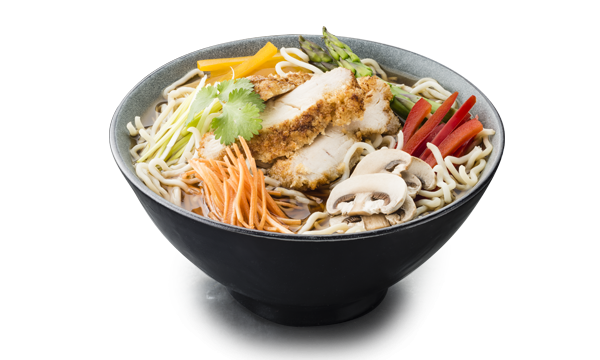
\includegraphics[width=0.5\textwidth]{ramen}
    }
    \begin{itemize}
        \item<3-> Tous les phénomènes sociaux ne sont applicables à tous les individus à toutes les périodes.
        \item<4-> La vérité n'est pas toujours objective!
    \end{itemize}
\end{frame}

\begin{frame}{La sociologie positiviste}
    \begin{block}{Autres considérations}
    \end{block}
    \begin{itemize}
        \item Les expériences subjectives sont également valides, importantes et peuvent aussi être étudiés.
        \item Nous ne pouvons pas généraliser cela à l'ensemble des individus et trouver la vérité avec un grand V.
        \item Mais nous pouvons nous intéresser à comment différentes tendances émergeant des différentes expériences subjectives individuelles pour former les structures qui composent notre monde social.
    \end{itemize}
\onslide<2>\textbf{La subjectivité} c'est la signification que les individus donnent à leur expériences vécues.
\end{frame}

% \begin{frame}{Les donnés}
% \begin{block}{Les types de collecte de donnés}
%     \begin{itemize}[<+->]
%         \item[\faVials] Expériences
%         \item[\faUserFriends] Entretiens
%         \item[\faPeopleArrows] Observations
%         \item[\faDatabase] Données existantes
%     \end{itemize}
% \end{block}
% \end{frame}
% Exercice données
% types de données -> identifier population/échantillon

\section{\faFlask~Pratique}

\begin{frame}{Questions, méthode et données}
    \begin{block}{Exercice préparatoire}
    \begin{enumerate}[<+->]
        \item[\faBrain] Identifiez les concept importants liés à votre projet
        \item[\faProjectDiagram] Dessinez un diagramme causal des relations entre les concepts
        \item[\faChalkboardTeacher] Présentez!
        % \item Identifiez des types de données permettant de mesurer vos concepts
    \end{enumerate}
    \end{block}
\end{frame}

\section{\faLaptopCode~Technique }

\begin{frame}{\faLaptopCode~Technique}
    \begin{block}{Let's play!}
    \begin{enumerate}
        \item Téléchargez et installez \faRProject
        \item Téléchargez et installez RStudio
        \item Téléchargez et installez \LaTeX
        \item Lancez RStudio
        \item Let the fun begin ... \faMagic
    \end{enumerate}
    \alert{Tous les liens sont dans le syllabus.}
    \end{block}
\end{frame}

\maketitle

\end{document}
